\pdfoutput=1 
\documentclass[a4paper,12pt]{article}

\usepackage{graphicx}% Include figure files



\graphicspath{{./Figures/}}
% packages
\usepackage{comment}
\usepackage{amsfonts}
\usepackage[dvipsnames]{xcolor}
\usepackage{placeins}
\usepackage[perpage]{footmisc}
\usepackage[normalem]{ulem}
\usepackage{caption}
\usepackage{makecell}
\usepackage{subcaption}
%\usepackage{subfig}
\usepackage{jinstpub} 
\usepackage{multicol,tabularx,capt-of}
\usepackage{hhline}
\usepackage{booktabs}
\usepackage{multirow}
\usepackage{lineno}
\usepackage{xfrac}
\usepackage{url}
\usepackage{soul}
\usepackage{hyperref}
\usepackage{chemformula}

\usepackage[binary-units,separate-uncertainty=true]{siunitx}
\usepackage{mathtools} 
%\usepackage{amssymb}
\usepackage{physics}
\usepackage[colorinlistoftodos, textsize=tiny, obeyFinal]{todonotes}





\title{ A Robust High Voltage feedthrough for cryogenic systems}

\author[a,1]{J.Doe,\note{Corresponding author}}


\affiliation[a]{SLAC National Accelerator Laboratory,\\ Sand Hill Rd. Menlo Park, Ca, 94025, USA}
\affiliation[b]{Michigan State University,\\ 426 Auditorium Rd. East Lansing, Mi, 48824, USA}


\abstract{Conventional liquid noble gas time projection chambers (TPCs) consist of discreet field-shaping rings between a cathode and an anode, to maintain a uniform electric field throughout the drift volume. 
	The field-shaping rings are connected by a resistor chain to gradually reduce the voltage, approximating a linear potential gradient. 
	Here, we present a novel alternative approach to HVFT
	We report studies of the electrical properties of  performed in several apparatus. 
	We find that the resistance dependence is exponential with the square root of the temperature, resulting in an increase in the resistivity of by an order of magnitude when cooled to \SIrange{77}{90}{\kelvin}. 
	We also find that the dependence on the applied voltage follows the hopping-transportation model, with an exponential decay with respect to the square root of the electric field.} 



\keywords{cryogenic detectors}

\begin{document}
\listoftodos
\maketitle




\section{Introduction}
\label{sec:intro}
\subsection{Motivation}

\subsection{SLAC liquid argon test stand}

\begin{figure}[ht]
	{\includegraphics[width=0.6\linewidth]{inside_rans.jpg}}
	{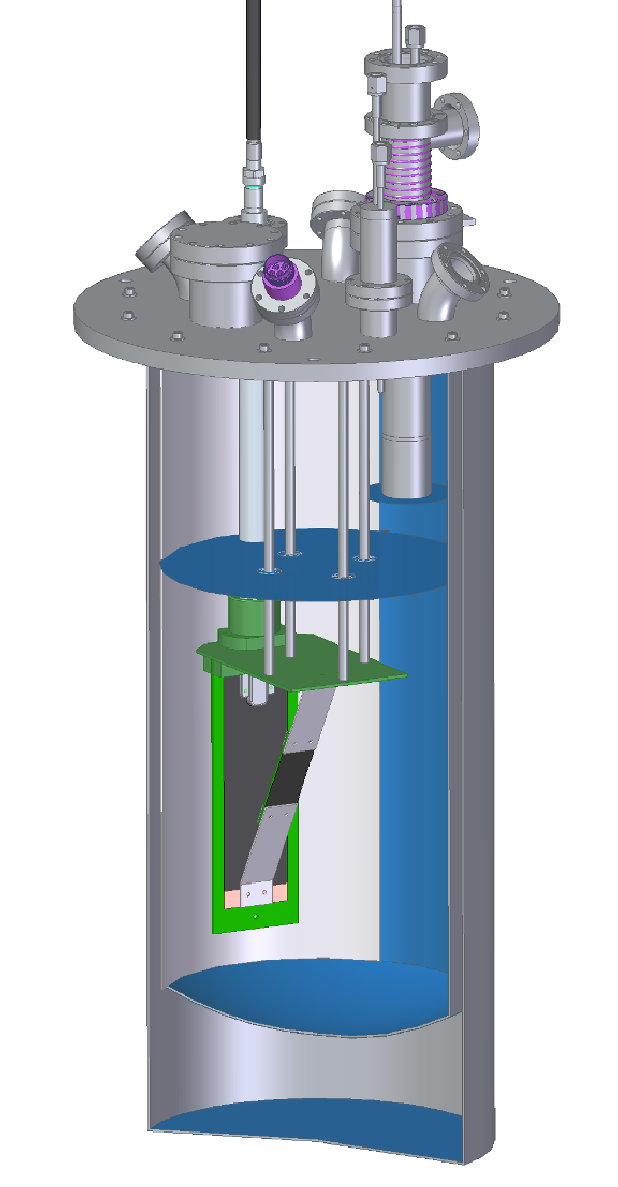
\includegraphics[width=0.42\linewidth]{rans.png}}
	\caption{(Left) A photograph of the LAr test assembly.
		The white tube is a polytetrafluoroethylene dielectric shield for the high voltage feedthrough that connects to a stainless port in the top of the dummy cathode. 
		The sample is mounted at an angle between the base of the cathode and a ground point on the fiber glass support structure. 
		(Right) A CAD of the LAr test stand. 
		The blue surface is the liquid level. 
		The cylinder on the right is a thermosyphon used to provide cooling.}
	\label{fig:full_sys}
\end{figure}



\section{Discussion and Conclusions}
\label{sec:sum}


summary

\section{Acknowledgment} 



\clearpage
% ========================================================================
% bibliography
% ========================================================================
%\printbibliography
\bibliographystyle{JHEP}
\bibliography{HVFTBib}

\end{document}